\chapter{Synthèse sur FPGA}

Dans ce chapitre, nous présentons la synthèse de descriptions VHDL. Notre cible est un circuit FPGA, embarqué sur une carte électronique.
Dans notre cas, nous utiliserons un FPGA Nexys4DDR de la société Xilinx, implanté sur une carte Digilent.

\section{FPGA : un circuit reconfigurable}
\paragraph{Définition d'un FPGA} Un FPGA est l'acronyme de \textit{field programmable gate array}. C'est un circuit numérique qui peut être vu comme un vaste receptacle d'équations logiques de de bascule D.
Un FPGA peut désormais en contenir plusieurs millions. Mais le plus intéressant tient au fait que les FPGA sont des circuits reconfigurables :
cela signifie qu'ils peuvent être reprogrammé à volonté. Cette "reprogrammabilité" leur confère des traits généralement associés au domaine du logiciel,
(s'exécutant sur un processeur versatile par nature). Les FPGA ont donc des caractéritiques de performances (dûes au parallélisme des équations fonctionnant simultanément)
et de reprogrammabilité.\\

% \begin{center}
%  \centering
%  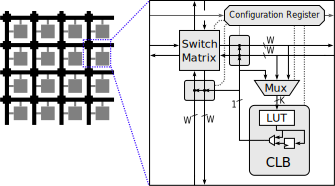
\includegraphics[width=8cm]{./figures/fpga_arch.png}
% \end{center}

\begin{figure}[h!]
  \centering
  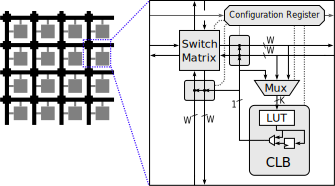
\includegraphics[width=8cm]{./figures/fpga_arch.png}
  \caption{Architecture des FPGA : routeurs, BLE, connection box et configurations}
  \label{fpga_arch}
\end{figure}

\paragraph{Architecture interne}
L'architecture d'un FPGA se présente comme un réseau à deux dimensions \footnote{Des travaux de recherche avancés proposent la 3D...}
de blocs configurables appelés CLB (\textit{configurable logic blocks}) interconnectés par des \textit{routeurs} (ou matrice d'interconnexion ou \textit{switch matrix}).
\footnote{Ces CLB ont été inventés par Page et Peterson en  1985}. Ils sont eux-mêmes constitués d'une \textit{Look-up table} (LUT) à $n$ entrées : c'est une mémoire
qui permet d'enregister les valeurs attendues de n'\textit{importe quelle fonction booléenne de $n$ entrées}. C'est l'équivalent d'une petite table de vérité.

% \begin{center}
%  \centering
%  \includegraphics[width=8cm]{./figures/LUT4.png}
%  \caption{Architecture d'une table de lookup à 4 entrées (LUT4)}
% \end{center}

\begin{figure}[h!]
  \centering
  \includegraphics[scale=0.4]{./figures/LUT4.png}
  \caption{Architecture d'une table de lookup à 4 entrées (LUT4)}
  \label{fig:lut4}
\end{figure}

Ces éléments (routeur, connexion box, LUT) sont présentés succintement sur les figures \ref{fig:lut4} et \ref{fig:router}

\begin{figure}[h!]
  \centering
  \includegraphics[scale=0.4]{./figures/switch_box_directional.png}
  \caption{Architecture d'un routeur}
  \label{fig:router}
\end{figure}


\paragraph{Comparaison avec les ASICs} Pour rappel, les circuits logiques peuvent également être fondus sur des circuits d'un autre type : les ASICs.
Ces ASICs (application specific integrated circuits) sont plus performants que des FPGA en terme de densité de portes logiques, de consommation et de fréquence
d'exécution. Mais, comme leur nom l'indique, les ASICs ne sont pas fondamentalement reconfigurables (pour qu'ils le soient il faut les concevoir comme tels).
Ils visent des applications déterminées et fixées une bonne fois pour toutes. Le coût de fabrication complet d'un ASIC est prohibilitif dès lors que seul un
faible nombre de pièces sont sensées être produites : pour qu'il soit rentable, il faut viser plusieurs dizaines à plusieurs millions de pièces. A noter que
le coût brut du Silicium n'est pas le budget le plus important. C'est essentiellement la fabrication des {\it masques lithographiques} qui coûte cher.

Les FPGA ont tendance à s'opposer aux ASICs de ce fait. Toutefois, dans les faits,
FPGAs et ASICs se révèlent complémentaires : tout d'abord les FPGA permettent de {\it prototyper} tout ou partie des futurs ASICs,
dans des conditions proches du produit final (mêmes captures VHDL, mêmes chaînes de synthèse etc). Le coût à la pièce d'un FPGA
est plus élevé qu'un ASIC, mais sa disponibilité immédiate est intéressante. Certains domaines comme le militaire ou le médical profitent donc
avantageusement des capacités de FPGA.

\section{Flot de synthèse}

Le flot de synthèse que nous allons expérimenter est présenté sur le schéma suivant. A partir des sources VHDL et de contraintes diverses (mises en relation des entrées et sorties
des entités VHDL et des ports physiques du FPGA, etc), nous synthétisons un bitstream : c'est un fichier binaire capable de programmer le réseau précédemment étudié (CLB, configurations, Switch matrix etc).
Nous avons alors recours à un second outil, qui permet de programmer la carte effectivement.

\begin{figure}[h!]
  \centering
  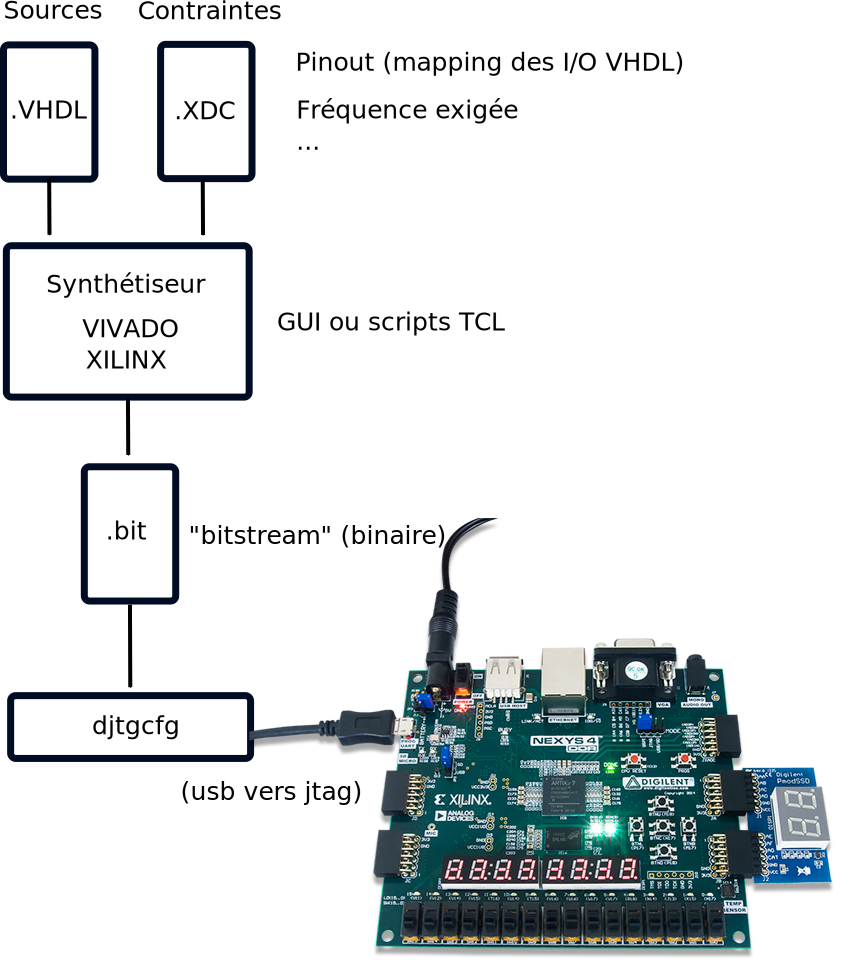
\includegraphics[width=8cm]{./figures/synthesis_flow.png}
  \caption{Aperçu du fLot de synthèse }
  \label{fig:flot_synthese}
\end{figure}

\section{Expérience pratique}
En séance de travaux pratiques, nous allons synthétiser un algorithme sur FPGA. Cet algorithme consiste à réaliser une multiplication par additions itérées, mais la démarche vaudrait pour un algorithme un peu
plus complexe. Pour passer à de "véritables" algorithmes, nous devrons nous doter de mémoires (non vues ici en première année) et d'un codage plus approprié que nos simples équations logiques : il faut passer
au niveau dit "RTL", où les équations logiques sont avantageusement remplacées par des constructions syntaxiques de VHDL, intuitives et automatiquement traduites en équations logiques par les outils (notion d'inférence).
Ceci sera étudié en deuxième année. Le présent exercice a tout de même l'intérêt de "démontrer" si besoin que nos équations logiques sont justes ! Tant les FSM que les chemins de données sont correctement réalisées avec des équations que nous
avons eu le mérite d'écrire et de simplifier "à la main".\\

La synthèse sur la cible FPGA Xilinx se fait à l'aide d'un script écrit par nos soins dans le language TCL. Ce langage pilote la plupart des outils de CAO moderne.
Ce script se lance en ligne de commande comme ceci :

\begin{lstlisting}[language=bash]
  $ vivado -mode tcl -source script.tcl
\end{lstlisting}

A l'issue de cette synthèse (qui peut durer plusieurs minutes), un fichier de bitstream est produit ({\it .bit}). C'est ce fichier qui configure le circuit FPGA final.
Le chargement du fichier sur la carte se fait ici par un cable USB entre le PC et la carte. Le chargement se fait à l'aide d'un outil logiciel fourni par Digilent.

\begin{lstlisting}[language=bash]
  $ djtgcfg prog -d Nexys4DDR -i 0 -f top.bit
\end{lstlisting}
Votre circuit est alors prêt à l'emploi !

%\section{Conclusion}
